\chapter{Design and Methodology}
\label{cha:design-and-method}


The Container monitoring system is designed as a Web of Things system using different communication paradigms. The System consists of several components, namely container sensor node, technician hand terminal and a central server. All of these components work together in order to inform the technician in the field as well as the surveilance personess about potential issues with shipping containers during transport. The communication links between different are clearly defined as REST, Bluetooth Low Energy advertising mode and WebSocket. The high level overview of the system is as follows:

\bigskip
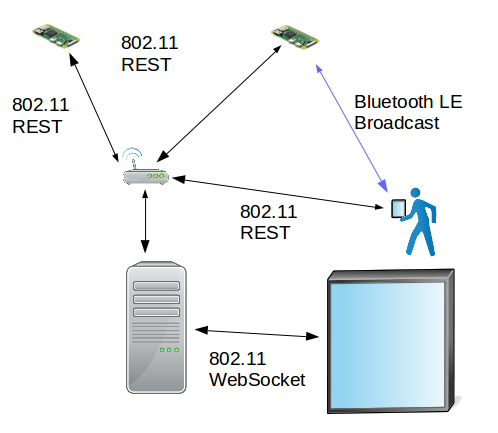
\includegraphics[scale=0.5]{gfx/overview}
\bigskip

The system can remain functional even without the central server in place, however alarm information is then not availble beyond simple alarm identifier. Here each individual component will be described as well as communication processes between the components.

\section{Sensor node}
\label{sec:sensor}

The sensor node is an embedded sensing device with ability to sense necessary phenomena for the shipping container. Once the phenomena has been sense it is able to compute simple actions on the sensed data and determine the state of the device as a result of this computation. The result, which can be and alarm or ok state (no alarms raised by the system) will then be transmitted out of the device in multiple ways: \newline
\begin{enumerate}
  \item Using Wireless communication, specifically Bluetooth Low Energy in order to communicate alarms to the hand terminal, once the hand terminal comes to the proximity (range of the Bluetooth Low Energy transmission) of the container.
  \item Using REST to communicate the alarm data to the central server, existing locally within the ship.
\end{enumerate}

\smallskip
The device also transmits its unique (within the ship) Identifier in order to pinpoint the source of the alarm. Processing on the device is as follows:\newline

\begin{figure}[!h]
  \centering\footnotesize\sffamily

    \begin{sequencediagram}
       \newthread{p1}{\normalsize sensor node}
       \newinst[1]{CS}{\normalsize central server}

       \begin{call}{p1}{getSensorReading()}{p1}{return SensorData}
       \end{call} 

       \begin{call}{p1}{calculateAlarm()}{p1}{return Alarm}
       \end{call}

       \begin{call}{p1}{broadcastBLEAlarm()}{p1}{}
       \end{call}

       \begin{messcall}{p1}{send alarm data}{CS}
       \end{messcall}

       \begin{messcall}{CS}{send reply}{p1}
       \end{messcall}
    \end{sequencediagram}
    \caption{Sensor node sensor data processing and alarm communication sequence}
    \label{fig:seqdia1}
\end{figure}

\smallskip

\section{Hand terminal}
\label{sec:terminal}

The hand terminal is a device that enables the technician to recieve and review alarms from containers as the technician comes to the proximity of the container raising the alarm. The hand terminal listens to the Bluetooth Low Energy broadcasts and shows potential alarm broadcasts on the screen. The alarm closest to the device is to be presented as the most pressing in order to lead the technician to handle the closest containers first. The device gets the alarm identifier from the sensor node, and the alarm description and possible resolution from the central server. The technician can decide to resolve the alarm on device which in turn must inform the central server about the resolution of the alarm (in order for all monitoring parties to know that the alarm has been resolved). The communication between the hand terminal and the central server uses REST. The hand terminal is designed as an Android application so it is usable on Android devices equipped with BLE chips. The hand terminal device defines several use cases for the technician:

\smallskip
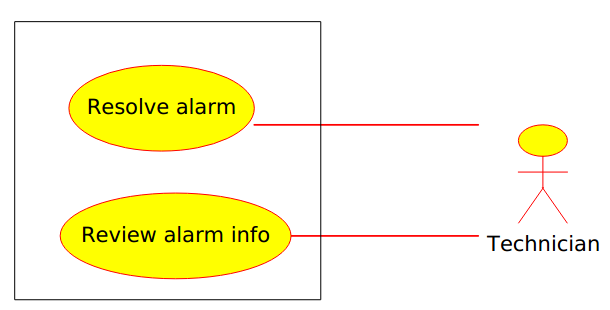
\includegraphics[scale=0.6]{gfx/handterminal}
\smallskip

The hand terminal computation and communication flow for alarm receiving and alarm resolution is as follows. Please note that all of the components of the system are involved:
\begin{figure}[!h]
  \centering\footnotesize\sffamily

    \begin{sequencediagram}
       \newthread{p1}{\normalsize sensor node}
       \newinst[1]{HT}{\normalsize hand terminal}
       \newinst[1]{CS}{\normalsize central server}

       \begin{messcall}{p1}{broadcast Alarm()}{HT}
       \end{messcall} 

       \begin{messcall}{HT}{get Alarm Info}{CS}{Alarm data}
       \end{messcall}

       \begin{call}{HT}{showAlarmMessage()}{HT}{}
       \end{call}

       \begin{call}{HT}{resolveAlarm()}{HT}{}
              \begin{messcall}{HT}{resolve alarm}{CS}
              \end{messcall}
              \begin{messcall}{CS}{send reply}{HT}
              \end{messcall}
       \end{call}

    \end{sequencediagram}
    \caption{Hand terminal handling receival and resolution of an alarm. The resolution is a technician action, hence it is not automatically executed at the alarm receival event.}
    \label{fig:seqdia2}
\end{figure}

\smallskip

\section{Central server}
\label{sec:server}

The Central Server is a component within the system that the surveillance personnel uses to get an overview of the global state of the system. This is the component of the system which provides data storage in regards to alarm definitions, users, sensor nodes as well as data storage for alarms generated by the sensor nodes of the system and alarm resolutions of alarms handled by technicians. This component also provides webhosting for a small webapplication that monitoring clients can connect to and get overview of the system. This application provides information about sensor values coming from sensor nodes and also alarms coming from sensor nodes. The central server must therefore communicate with different connected parties in multiple ways: \newline
\begin{enumerate}
  \item Provide a REST API that the sensor node(s) and hand terminals can use in order to provide their data and get necessary information.
  \item Provide a REST API as a basis for a small webpage that is used to display global data generated by the system.
  \item Provide a WebSocket connection that a web application client can connect to and obtain alarm information dynamically without the need for polling.
\end{enumerate}

These communication principles can be simply visualized as:

\smallskip
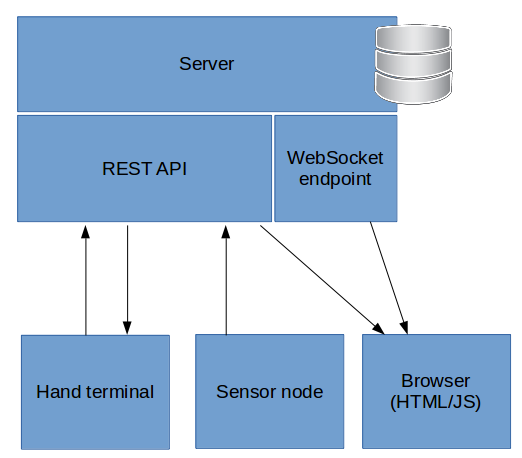
\includegraphics[scale=0.6]{gfx/servercomm}
\smallskip

The important part of the central server components is its data storage services as well. These are handled as follows:
\begin{figure}[!h]
  \centering\footnotesize\sffamily

    \begin{sequencediagram}
       \newthread{p1}{\normalsize sensor node}
       \newinst[1]{CS}{\normalsize central server}

       \begin{messcall}{p1}{send alarm}{CS}
       \end{messcall} 

       \begin{messcall}{CS}{send reply}{p1}
       \end{messcall} 

       \begin{call}{CS}{storeAlarm()}{CS}{return status}
       \end{call}
    \end{sequencediagram}
    \caption{Central server storing an alarm to the database}
    \label{fig:seqdia3}
\end{figure}

\smallskip

\section{Method}
\label{sec:method}

The method for creating of the system was based on identifying a problem -> refining a problem definition -> identifying the development process, implementation and validation. It has been determined that the system development will be done using agile principles where scheduling of development activities has been done dynamically based on their respective priority using a SCRUM board. Due to the nature of the system, different components could be developed in parallel with agreements necessary on data models and communication endpoints (interfaces). This was to enable rapid progress as well as ability to test different components independently during the development phase. The process was carried out iteratively and the steps involved were: \newline
\begin{enumerate}
  \item Determine subtasks related to components and add them to backlog.
  \item Determine priorities in ragrds to different subtasks and mark them accordingly.
  \item Select subtasks for implementation based on priority.
  \item Agree on interfaces between the parts of the components that are relevant to selected subtasks.
  \item Implement subtasks.
  \item Integrate the subcomponents if possible in the stage of development.
  \item Verify the implementation of subtasks.
\end{enumerate}

%%% Local Variables:
%%% mode: latex
%%% TeX-master: "../ClassicThesis"
%%% End:
